\section{Background}
Supercomputing is high-performance for data-intensive or compute-intensive tasks, e.g. deep learning training and big data processing. To meet the performance demands, supercomputing is generally constructed in a cluster which includes multiple machine instances. So, there are urge demands for network between instances in supercomputing. RDMA is a popular high-performance network in supercomputing. Meanwhile, to utilize the server resources, supercomputing is going cloud, especially hybrid virtual environments.

Virtualization for VMs and containers are in different spaces because of their characteristics. VMs need emulate whole virtual hardware environments for guest operation system with hypervisor (kernelspace). So, applications in VMs is isolated by guest OS with more security but higher overhead. Containers are shared with the host OS but with runtime isolation. So, containers have low overhead and fast boot-up time. For applications, the abstraction of VMs includes own kernel space and containers only includes own user space with shared host kernel space.


% RDMA: 
% RDMA网卡是控制和数据路径分离, RDMA网卡内部构造
% RDMA网卡数据传输机制,按门铃操作
RDMA (Remote Direct Memory Access) has hardware protocol stack and zero copy technology, so applications can bypass the kernel to read and write remote memory data, without the participation of remote CPU. As a result, RDMA has high throughput, low latency and low CPU load. Applications need to use Verbs interface when using RDMA. In Verbs, as shown in Figure~\ref{fig:rdma-feat}, RDMA is separate control path and data path. The former is the management about RDMA context, mainly including lots of RDMA resources, such as Queue Pairs (QPs), and Memory Regions (MRs). the operations like ibv\_create\_qp, reg\_mr; The latter is the usage of RDMA context and resources, which is the data commands like ibv\_post\_send and ibv\_post\_recv. In a RDMA workflow, the communication is based on Queue Pair (QP). The application writes the RDMA work request to the QP, and then ``press''  the RNIC's doorbell register, which is mapped to application when context init, and the RNIC's hardware processor will execute the work request in the QP to forward data. For applications, the entire operator is in the user space.

\begin{figure}[!ht]
	\centering
	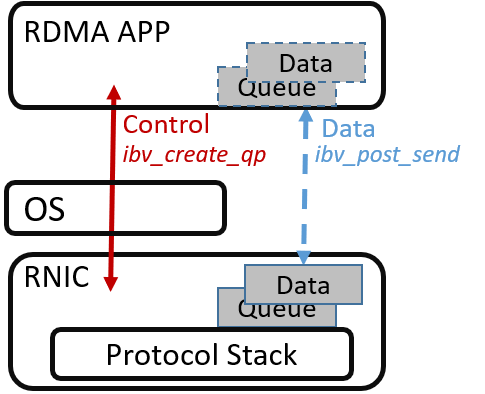
\includegraphics[width=0.6\linewidth]{images/rdma-feat}
	\caption{Native RDMA Feature}
	\label{fig:rdma-feat}
\end{figure}


